



\chapter{Conclusion -- Evolved strategy of Yersinia Pestis}












The main finding across all of the (see appendix B) above cases (specifically, where the total replicative ``rate-density'' remains fixed between comparrisons), both in the continuous time and discrete time cases, is that the mean of the process at the end of the specified period is identical.  How it gets there varies, along with what happens after. Also, the variance and distribution seems to vary.  But the point remains -- early replicative enphasis given constant overall "potential replicative density", gives no advantage over a specified period, to the expected overall growth. \ 
Of course, this assumption of eqivalent "replicative density" does not apply to the case of comparrison between complete etracellular growth when set against the alternative of an initial "replicative boost" in macrophages. 











\subsection*{Two common exceptions to this rule}

\subsubsection{Non-conservation}
Non-finite supply of replicative means. Basically when the key assumption is removed. Perhaps a higher replication rate is accessible at larger population sizes.



\subsubsection{Monopoly effect}
Matthew effect






In appendix B, there is a summary of some work witch mathematically demonstrates a property of branching. That articifially front weighted replicative advantage --- when assuming an overall constant "replicative potental" --- does not give any advantage to a process with regards to its expected growth. In more intuitive terms, say a bacterial population had access to a finite supply of food on an agar plate, if it was to use more of it towards the beginning, and less later, there would not be any advantage to its overall expected growth. This seems relatively obvious, but I just wanted to check, and the maths checks out. At least in the mean. When it comes to the variance and distribution of outcomes, there is some nuance,  but let us leave this aside. \par 

What of the case of plague finding early replicative in macrophages? The condition of constant "replicative potential" does not apply when comparing with the case of less fecund extracellular replication. 




\section{Two phase}



Thinking about the replication of Yersinia pestis within the body. There are two distinct phases in its pathogenesis. Namely, the preinflamatory and the postinflamatory periods.To recall,  in the first of these, YP replicates mostly intracellularly within macrophages. Then, as the body recognizes the alien presence and mounts a neutrophil attack, YP switches to extracellular replication. 

Due to the fact YP doesn't begin with extracellular replication, it seems sensible to assume that there is an advantage to living within macrophages. As a rudimentary model of this behavior, we can take in simple terms that the replication rate is higher in this proinflammatory phase. That viral multiplication is easier within the macrophage intracellular environment. 

In the cell there are fewer of the extracellular mechanisms of innate immunity: thinking specifically about complement and bacteriophages. 

Perhaps there is an adaption to the specific presentation of bacteriophages in a particular host on the time scale of YP infection dynamics. That is, within only a handful of replication cycles, small variations to the bacteria cause the population to gain resistance to these host-specific bacteriophages. 

Such a dynamic could be captured with a model using the two phases, but with a decaying death rate in the second extracellular phase
$\mu(t) = a + a\ee^{-t}$. If we were to take this process individually. That is with some initial count of replicators undergoing only this second phase. Given the decaying death rate, there may be an initial period in which replication is subcritical. And in this case, the size of the initial population would become vitally important to whether the infection persists.







\subsection{Host to host Galton Watson process}



Consider a host-to-host branching process in which the dynamics are a basic Galton-Watson process with probability $p$. But that $p$ is defined by a within-host dynamic. Essentially, if the infection within the host attains a threshold bacterial load, the infected person will infect two more people. If it does not and gets killed off by the immune system, no further infections will result from that individual. Thus, the replication probability, $p$, results from the chance of this happening; of the infection persisting and ascending to a high infectious load. \par

The simplest version of this would be a simple birth-death process and a defined threshold value.  We are then interested in the probability of the process ``hitting'' one threshold or the other (either the upper positive threshold, or 0), and this is the replication probability.\par

Then, we are in a position to compare different models. Especially, the two-phase models (with and without variable death rate). It will be straightforward to show that probability of ``host-to-host transmission''  (reaching the threshold) will be greatly altered by the inclusion of this initial phase. The time at the beginning when YP temporarily exploits the within macrophage environment to gain an early advantage. This early advantage being of vital importance to the outcome from the onset of the second phase. 






\subsection{Two phase PGF}

For reasons soon described, we are really only interested in the overall extinction probability, but this is the starting point. 


$$G^{(\text{whole-process})}(x,t)    = \begin{cases}
G^{(\text{phase-1})}(x,t), & t< t_c\\
\sum_{k=0}^\infty   \pr{\xx_{t_c}^{(\text{phase-1})} = k} \lrb{G^{(\text{phase-2})}(x,t-t_c)}^k, & t>t_c
\end{cases} 
$$


$$ \pr{\xx_{t_c}^{(\text{phase-1})} = k}   =  \lrb{k!}^{-1}  G^{(phase-1)}_{kx}(0, t_c)$$




There are two phases. The second is a birth death process that is only slightly supercritical, $\beta > \mu$ but $\beta \approx \mu$. The first is a BDC process for which $\lambda >> \mu$ (favours replication). The first phase represents the intracellular phase of an infection, second, the extracellular phase.\par

Consider the situation of an infected individual. Assume they will either go on to infect two more individuals, or they will recover and the infection will die with them. In this way, a Galton Watson style epedemic takes place. Suppose the former case takes place with probability $p$. Then, the expected number of infections caused is $2p$. Now, whether the person infects others will depend on the success of the infection within them.\par

In a birth death process, which the within-person infection can crudely be modelled as, if the process is supercritical, it will either blow up, or die out. Ceasing eventually with some probability, $p_0$. Lets say that the person goes on to infect in the case that the infection does not cease (blows up in the simplified BD model), happening with probability ($1-p_0$). In this way $p = 1-p_0$.\par

So take the second phase outcome as the deciding factor. The probability that the infection in the second phase wont cease will depend on what happens in the first phase. That being a BDC process, we can compute $p_0$ of the second phase with the following formula (law of total probability)

$$p^{\text{whole-process}}_0 = \sum^{\infty}_{k=0} \pr{\mathcal{K} = k} \lrb{p_0^{(\text{phase-2})}}^k$$ 

$$p_0 = b + \sum^{\infty}_{k=1} \frac{\delta}{\lambda} \lrb{\frac{1}{a}}^{k} \lrb{\frac{\nu}{\beta}}^k$$ 


$(\nu/\beta)^N$ being the probability of eventual extinction of a standard BD. Note, the first phase BDC uses $\lambda$, $\mu$ and birth/death rates; the second phase BD process uses $\beta$, $\nu$. The $b$ term comes in at the $k=0$ case (probability of death in first phase BDC). \par
Hence, the probability of infecting another two people is $p = 1-p_0$. And the $R_0$ number of this Galton-Watson epidemic is

$$ \mean{Z} = 2p = 2\lrb{1 -  b + \sum^{\infty}_{k=1} \frac{\delta}{\lambda} \lrb{\frac{1}{a}}^{k} \lrb{\frac{\nu}{\beta}}^k} $$


The question is, how does this value depend on the dynamics of the first phase. On the expected burst size and time, these depending substantially on the catastrophe rate, $\delta$. 


The above formula is for the BDC to birth death case.  One of a few choices of model:

\begin{itemize}
\item BD - BD
first BD higher effective replication ratio (goes on for some defined time)
\item BDC - BD
BDC higher replication rate (goes on for time dictated by cat rate)
\item Const - BD
\item Const - BD (subducive) To represent the host bacteriophage adaption hypothesis. 
\end{itemize}

\noindent


\begin{figure}[H]
    \centering
    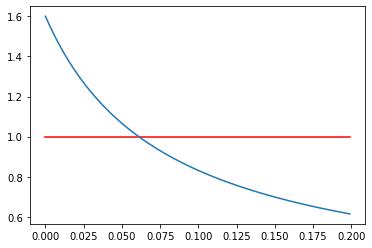
\includegraphics[width=0.5\textwidth]{chapter9/IMG_ch9/rough.png} % Adjust the width as needed
    \caption{ $(\lambda, \mu) = (1, 0.2)$ in the first phase, and $(\beta, \nu) = (1, 0.9)$. This is the host-to-host GW proliferability measure ($\mean{Z}$) in the BDC to BD case. The plot shows $\mean{Z}$ plotted against $\delta$. What is shown is that for supercritical epidemic spread (under the given assumptions), the initial phase of infection in macrophages should produce a sufficient bacterial load to overcome the likelihood of extinction in only near-supercritical growth in the extracellular phase. This is a consequence of $\delta$ being sufficiently small. That is, the propensity for the macrophage to burst being low permits a higher expected release in this crucial initial phase.}
\end{figure}



\begin{figure}[H]
    \centering
    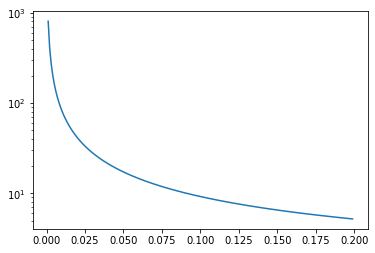
\includegraphics[width=0.45\textwidth]{chapter9/IMG_ch9/rough2.png}   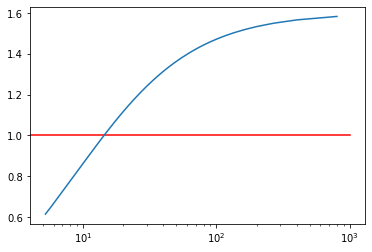
\includegraphics[width=0.45\textwidth]{chapter9/IMG_ch9/rough3.png} % Adjust the width as needed
    \caption{Left: mean burst size as a function of catastrophe rate $\delta$.  Lower propensity to burst, higher burst size.
Right: GW epidemic replication number $\mean Z$ plotted against mean burst size. High burst size, greater chance of the infection surviving the minimally supercritical pro-inflammatory phase, higher probability of not going extinct, and thus growing exponentially, causing host-to-host proliferation.}
\end{figure}








\section{Quadrant argument}





To begin  understanding YP's particular invasion strategy, we can start by painting a schematic picture of the circumstances it comes up against in the body. For some reason YP has evolved to at first grow intracellularly, then transition to primary extracellular replication. Let us simplify
 the case of intracellular replication to being within either macrophages or neutrophils only (ignoring for simplicity the presence of dendritic cells, eosinophils, basophils and mast cells. Though these are no doubt also relevant in reality). We can make the simple assumption that the within-neutrophil environment is more hostile to YP than that of Macrophages. 

Macrophages are the run of the mill, generalist leukocyte whereas neutrophils are more specialist killers. As I understand it, it is mainly neutrophils that are recruited and released on mass in response to recognition of such a bacterial infection as YP.  

If we took YP replication to be a simple BD process, this assumption would be reflected in the death rate within neutrophils being higher than that within macrophages. There is the complication discussed previously where killing within leukocytes has something to do with granules (neutrophils
 have more of these). This producing the aforementioned non-autonomous effects. But here, it seems sufficient to gloss over this underlying reality to take the death rate as merely fixed. 

So $\mu_N > \mu_M$. What about $\mu_E$, the extracellular death rate. I want to put forward the supposition that this is somewhere in between the two. That the situation outside of cells is relatively more hostile than within macrophages, and relatively less than within neutrophils. 
The argument for this assumption is that if there was no advantage to being within macrophages, it seems unlikely that YP would have evolved to exploit their intracellular environment at all. And, if there was an advantage to being within neutrophils (over the extracellular environment), it begs the question why phagocytosis would
 be resisted when a swarm of these hosts presents itself. Hence, let us proceed with the assumption 
$$\mu_N > \mu_E > \mu_M$$

with each of the three environments exhibiting standard birth-death dynamics with equal birth rate,
$$\beta_N = \beta _E = \beta_M.$$
This itself is an assumption that begs some justification. There may be variation among these replication rates; in reality, differing supply of nutrients and energy within cells may cause faster generational production. But for the present argument, it seems best to take them as equal so as not to introduce unnecessary complication. And anyway, the distinction of key importance is the overall effective replication rates, $\beta_i - \mu_i$. 


\vspace{10pt}
\hrule
\vspace{10pt}

\noindent
\textbf{Aside:}  There are other explanations for why YP might initially favour macrophage absorption. Especially, the possibility that macrophages are merely used as a transport mechanism for YP to get to the Lymph nodes which probably have a greater supply of food.\par
It is also possible that the initial pro-phagocytosis phase is a lingering hangover from the time the bacteria lives within a flea. 
For now, we will ignore these genuine possibilities to explore the argument that there might be a more fundamental strategic advantage. 

\vspace{10pt}
\hrule
\vspace{10pt}

\noindent
Following pathogen recognition, the body recruits neutrophils and delivers them to the site of infection. In a simplified framework, we can model this by there being a stepwise increase in neutrophils at a defined time, $t_N$, following the onset of infection. In reality, the fact that YP ``hides'' within macrophages could act to delay the onset of neutrophils. This would manifest in our model at $t_N$ changing according to the bacteria choice of strategy. But this detail can be ignored for the present argument, because whether it is advantageous for YP to be absorbed or not does not here depend on the time at which the neutrophils arrive. 


The bacteria to gain the best proliferative advantage will need to maximise its effective replication rate, $\beta_i - \mu_i$. Its evolutionary process has been able to select for whether to accept or resist phagocytosis at stages of the infection, but we will take it that the bacteria can not discriminate between absorption by macrophages and neutrophils. 


Because  $\mu_N > \mu_E > \mu_M$ and $\beta_N = \beta _E = \beta_M$, it follows that
$$\beta_M -  \mu_M > \beta_E -  \mu_E >  \beta_N - \mu_N.$$
Macrophages offer the best replicative opportunity. But because we assume YP can not differentiate between macrophages and neurtophils, the expected replicative rate for each strategy will depend on the probability that absorption is executed by a macrophage over a neutrophil. In the case of a pro-phagocytosis strategy, let us take the probability of macrophage absorption as $p_M$; $p_N$ for neutrophils. If we also assume that one of these outcomes is certain, it follows that $p_M = 1 - p_N$. These probabilities resulting from the ratio between neutrophils and macrophages present, 
$$p_M = \frac{\# M}{ \#N + \#M}, \quad p_N = \frac{\# N}{ \#N + \#M}.$$
with $p_N$ increasing at time $t_N$. \par
The mean effective replication rates for each strategy will hence be as follows:

\begin{itemize}
\item \textbf{Pro-phagocytosis}: $R_{\text{pro}} = p_M(\beta_M -  \mu_M) + p_N (\beta_N - \mu_N)$
\item \textbf{Anti-phagocytosis}: $ R_{\text{anti}}  = \beta_E -  \mu_E $ 
\end{itemize}
And with some rearrangement, the former becomes
$$ R_{\text{pro}} =(1-p_N)(\beta_M -  \mu_M) + p_N (\beta_N - \mu_N)$$
$$R_{\text{pro}} =p_N \lrbs{ (\beta_N - \mu_N)  - (\beta_M -  \mu_M)}  +     (\beta_M -  \mu_M).$$

\noindent
Pro-phagocytosis will cease to be a favourable strategy when 

$$R_{\text{anti}} > R_{\text{pro}}$$ 

\noindent
which occurs when the proportion of neutrophils, $p_N$, increases beyond a threshold: 

$$p_N > \frac{ (\beta_M -  \mu_M)  -  (\beta_E -  \mu_E) }{   (\beta_N - \mu_N)    -   (\beta_M -  \mu_M) } .$$

\noindent
Noting that $\beta_N = \beta _E = \beta_M$, this becomes

$$p_N > \frac{  \mu_E - \mu_M }{    \mu_M - \mu_N} .$$

\noindent
Given this threshold is crossed with the onset of the neutrophil influx at time $t_N$, an argument would be satisfied for why YP has evolved to switch between the two strategies. 

 




\section{Public good accumulation --- a model,  and potential relevance to Y. pestis}

Matt Asker, Lluis Hernandez and Mauro Mobilia work in the field of antimicrobial resistance \cite{asker2023coexistence}.    Cancerous cells exhibit two varieties: those resistant to a drug, and those succeptible. The resistant ones produce a substnce which they expell into their surrouning matrix. It's called a public good because it facillitates the resistance of all cancer cells to the drug, both the resistant and suceptible types. \par 
It occured to me that there may be something similar going on with Y. pestis in macrophages. -- This is purely my speculation, and may not at all be the case, but even if it isn't, the dynamics may be interesting in and of themselves.  -- Y. pestis has evolved resistance to the toxins that are presented within macrophages.  It occured to me that if Y. pestis were to execute this resistance using a "public good" substance,  that it would be confined within the resident macrophage and thus concentrated, rather than being dispersed.  Something like this could further support the argument that the within-macrophage environment provides a replicative advanage (assuming there are also toxins and other challenge factors (possibly bacteriophages) in the extracellular space). 


\begin{figure}[H]
    \centering
   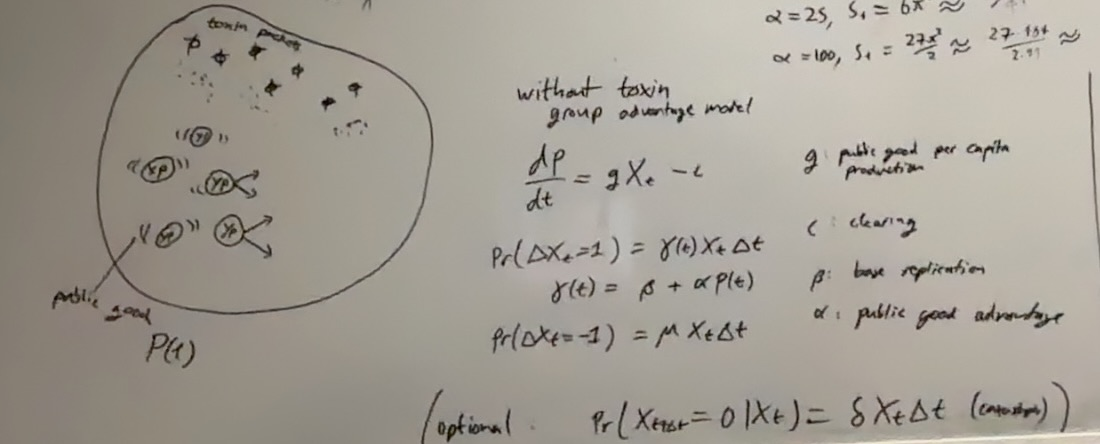
\includegraphics[width=0.99\textwidth]{chapter9/board.jpeg} % Adjust the width as needed
    \caption{Y.  pestis represented within a macrophage along with toxin containing packets.  Public good, $P(t)$ is produced by }
\end{figure}


\subsection*{Model for public good replication without directly accounting for toxic granules}

The effect of the toxic immune substance can be incorporated into the linear death rate.  Of course, this overlooks the dynamics of toxin depletion as discussed in chapter 6,  but it seems good in the interest of simplicity.  And the point of focus is the dynamics of this public good.  Let us make the simplified assumption that the presence of the "public good" increases the replication rate ($P(t)$: public good concentration; $\xt$: Y. pestis bacteria): 


$$\ddt{P} = g \xt - c,$$
$$\pr{\Delta \xt = 1} = \gamma(t)\xt\Delta t + o(\Delta t),$$
$$\gamma(t) = \beta + \alpha P(t),$$
$$\pr{\Delta \xt = -1} = \mu \xt \Delta t.$$

\begin{itemize}
\item[$g$:] public good production rate
\item[$c$:] public good clearing rate
\item[$\beta$:] base birth rate
\item[$\alpha$:] public good advantage
\end{itemize}
It might well make more sense for the presence of public good to reduce the death rate rather than increase the birth rate.  Another formulation could be thought up along these lines. \par 

\subsection*{Potential quantity of interest}

Suppose we consider a successive version of this process for which in the case of late time non-extinction it is assumed that the infected cell dies and infects two more cells.  A simplification which creates a sort of Galton Watson process in which the division probability is subject to embedded dynamics.\par 
In this case,  for the overall GW process to be supercritical,  the probability of within-cell non-extinction must be greater than one half.  We could as the question of what would be the minimum required incident cohort size into a cell to achieve this,  especially in the case where $\mu > \beta$, in which the public good plays a critical role.  In other words, 

$$\text{inf}\{K : \lim_{t\to\infty}\lrb{\pr{\xt > 0 | \xx_0 = K }}\} = \text{?}$$
This could be computed numerically. 


\subsection*{Notes -- public good in a closed group}

What if there is some replication advantage to a cohort of Y. pestis bacteria living within the enclosure of a macrophage; and what if there is something like a public good produced by the bacteria, and confined within the boundary of the host cellular membrane -- this underpinning a benefit of within group (macrophage) cooperative co-existence. \par 

\vspace{10pt}
\noindent
Something that comes to mind is,  as in other cases of cultural practice,  in Jewish communities it has historically been virtuous to cooperate within the community whilst facing outwards with more competitiveness.  In Shakespeare's "The merchant of venice" it is revealed that at the time (16h CE) it was forbidden for Jews to lend money with interest within the community,  whilst being acceptable to do so with Christians. \par

\vspace{10pt}
\noindent
Just like the individual is rewarded -- paid by gains of cooperative advantage - for being effective to the purpose and success of the private group; so the private group can be rewarded for benefiting circles of wider scope.\par 
And going in the other direction, the individual within the individual is crucial in its avarice when chasing personal enterprise. \par 
Surely these things don't need to be contradictory. 



%My feeling is that somewhere in all this is a helathy middle ground between the two extremes of a particular ideological spectrum.  Crudely,  that between the socialist and the individualistic libertarian capitalist.  On the one hand we have everyone driven to povery by the abolition of accute progress; on the other hand, we have the pathology of extreme inequality.  Something in the middle might see a framework of nested groups internally cooperating and externally competing. 



















































































































%%%%%%%%%%%%%%%%%%%%%%%%%%%%%%%%%%%%%%%%%%%%%%%%%%%%%%%%%%%%%%%%%%%%%%%%%%%%%%%%%%%%%%%%%%




















%%%%%%%%%%%%%%%%%%%%%%%%%%%%%%%%%%%%%%%%%%%%%%%%%%%%%%%%%%%%%%%%%%%%%%%%%%%%%%%%%%%%%%%%%%

